\begin{equation*}
% the copies of the shared address a are drawn double: expanding the term repeats it, once per summand
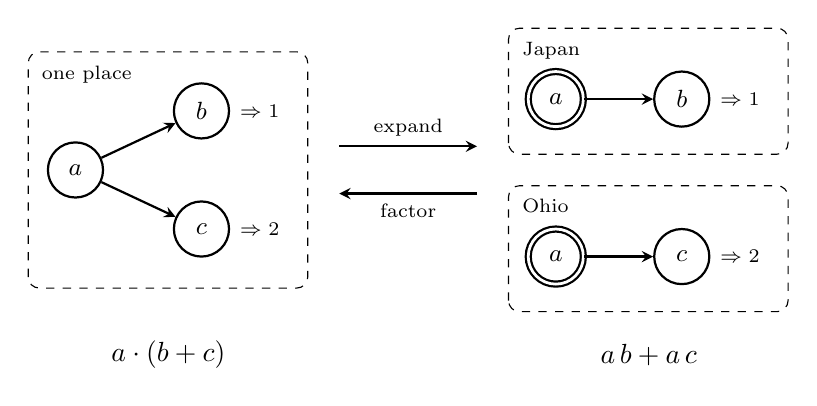
\begin{tikzpicture}[
  seg/.style={draw, circle, thick, minimum size=7mm, inner sep=0pt, font=\small},
  copy/.style={seg, double, double distance=1pt},
  hop/.style={thick, ->, >=stealth},
  place/.style={draw, dashed, rounded corners=4pt},
  note/.style={font=\scriptsize}
]
% colocated: a.(b + c), one object at one place
\draw[place] (-0.6,-1.5) rectangle (2.95,1.5);
\node[note, anchor=north west] at (-0.55,1.45) {one place};
\node[seg] (a) at (0,0) {$a$};
\node[seg] (b) at (1.6,0.75) {$b$};
\node[seg] (c) at (1.6,-0.75) {$c$};
\draw[hop] (a) -- (b);
\draw[hop] (a) -- (c);
\node[note, anchor=west] at (b.east) {$\Rightarrow 1$};
\node[note, anchor=west] at (c.east) {$\Rightarrow 2$};
\node at (1.18,-2.35) {$a \cdot (b + c)$};
% expanding and factoring
\draw[hop] (3.35,0.3) -- node[note, above] {expand} (5.1,0.3);
\draw[hop] (5.1,-0.3) -- node[note, below] {factor} (3.35,-0.3);
% placeable apart: a b + a c, two objects that two places may hold
\draw[place] (5.5,0.2) rectangle (9.05,1.8);
\node[note, anchor=north west] at (5.55,1.75) {Japan};
\node[copy] (a1) at (6.1,0.9) {$a$};
\node[seg] (b1) at (7.7,0.9) {$b$};
\draw[hop] (a1) -- (b1);
\node[note, anchor=west] at (b1.east) {$\Rightarrow 1$};
\draw[place] (5.5,-1.8) rectangle (9.05,-0.2);
\node[note, anchor=north west] at (5.55,-0.25) {Ohio};
\node[copy] (a2) at (6.1,-1.1) {$a$};
\node[seg] (c2) at (7.7,-1.1) {$c$};
\draw[hop] (a2) -- (c2);
\node[note, anchor=west] at (c2.east) {$\Rightarrow 2$};
\node at (7.28,-2.35) {$a\,b + a\,c$};
\end{tikzpicture}
\end{equation*}
